\documentclass[12pt,a4paper]{report}
\parindent =0cm
\usepackage{amsmath}
\usepackage{amssymb,amsfonts, 
latexsym,cancel}
\usepackage{array}
\usepackage{bm}
\usepackage{float}
\usepackage{fancyhdr}
\usepackage{graphicx}
\usepackage{epstopdf}
\usepackage[colorlinks = true,
			linkcolor = black,
			citecolor = black,
			urlcolor = blue]{hyperref}
\usepackage{longtable}
\setcounter{MaxMatrixCols}{40}
\usepackage{multicol}
\usepackage{subfigure}
\usepackage{titling}
\usepackage{titlesec}
\usepackage{setspace}
\newcolumntype{E}{>{$}c<{$}}

\usepackage{anyfontsize}
\usepackage[utf8]{inputenc}
\usepackage{amsmath}
\usepackage{amsfonts}
\usepackage{amssymb}
\usepackage{makeidx}
\usepackage{graphicx}
%\usepackage{fourier}

\setcounter{MaxMatrixCols}{100}
\usepackage[left=0.1cm,right=2cm,top=2cm,bottom=2cm]{geometry}
\author{Guadalupe Monroy}
\begin{document}
\thispagestyle{empty} %% PARA QUITAR FORMATO DE PIES Y 
%\fbox{
\begin{minipage}[c][0.15\textheight][c]{0.17\textwidth}
    \begin{center}
        
\includegraphics[height=2.2cm, keepaspectratio=true]{imagenes/logocp} %% LOGO IZQUIERDO
    \end{center}
\end{minipage}
%}
%\fbox{
\begin{minipage}[c][0.15\textheight][t]{0.9\textwidth}
    \begin{center}
        {\scshape \Huge COLEGIO DE POSTGRADUADOS} %% NOMBRE DE LA UNIVERSIDAD
        \vspace{.5cm}   %% DEFINE EL ESPACIO ENTRE EL NOMBRE DE LA UNIVERSIDAD Y LA LÍNEA DOBLE
        \hrule height2.5pt  %% DEFINE EL ANCHO DE LA PRIMER LÍNEA
        \vspace{.1cm}    %% DEFINE EL ESPACIO ENTRE LAS DOS LINEAS
        \hrule height1pt  %% DEFINE EL ANCHO DE LA SEGUNDA LINEA (NORMALMENTE ES MAS DELGADA)
        \vspace{.4cm}   %% DEFINE EL ESPACIO ENTRE LA DOBLE LINEA Y EL NOMBRE DE LA DIVISIÓN
        {\scshape \LARGE  CAMPUS MONTECILLO}  %% NOMBRE DE LA DIVISIÓN
    \end{center}
\end{minipage}
%}

%\fbox{
\begin{minipage}[l][0.78\textheight][t]{0.1\textwidth}
    \begin{center}
    \hskip0pt
    \vrule width2.5pt height17cm    %% height definde la altura de la linea gruesa
        \hskip1mm
        \vrule width1pt height17cm  %% height define la altura de la linea delgada
        \end{center}
\end{minipage}
%}
%\fbox{
\begin{minipage}[c][0.78\textheight][t]{0.8\textwidth}
      \begin{center}
      \vspace{2cm}
        {\Large \scshape {PSEI-ESTADÍSTICA Y CIENCIA DE DATOS}}

        \vspace{2cm}

        \makebox[5cm][c]{\LARGE Examen. MODELOS LINEALES}  \\[16pt]
        PROFESOR DR. HUMBERTO VAQUERA HUERTA             \\[15pt]
        {\Large \textbf{{}}}\\[25pt]
        Al:\\[12pt]
        \textbf{ \Large {Guadalupe Monroy Hernández}}

        \vspace{2cm}
        
        \vspace{2.5cm}

        { Texcoco, Edo. México} \hskip2.5cm {}
      \end{center}
\end{minipage}
%}
\begin{enumerate}
%--------EJERCICIO 1------------
\item Considere los vectores en $R^2: y= \begin{pmatrix} -6 \\  4 \end{pmatrix},$ y $x = \begin{pmatrix} 3 \\  2 \end{pmatrix}$ \\ 

1. Encuentre: $<x,y>$, $||x||^2$, $||y||^2$

$<x,y> = x \cdot y = (-6)(3)+(4)(2)= -10$\\

$||x||^2 = (3)(3)+(2)(2) = 9 + 4 = 13$\\

$||y||^2 = (-6)(-6)+(4)(4) = 52$\\

2. Obtenga $cos \theta = \frac{<x,y>}{||x|| ||y||}$\\
\begin{align*}
    cos \theta & = \frac{<x,y>}{||x|| ||y||} = \frac{-10}{\sqrt{13} \sqrt{52}} = 0.9269
\end{align*}
3. Obtenga la proyección ortogonal del vector $y$ sobre la línea L expandida por el vector $x(\hat{y} = P_xy)$
\begin{align*}
    P_x (y) & = \frac{<x,y>}{||x||^2} x = \frac{(-6)(3)+(4)(2)}{3^2 + 2^2} \begin{pmatrix}
    3\\
    2
    \end{pmatrix} = \dfrac{-10}{13}\begin{pmatrix}
    3\\
    2
    \end{pmatrix} =\begin{pmatrix}
    -30/13\\
    -20/13
    \end{pmatrix}  
\end{align*}

4. Encuentre la distancia $x$ a L, es decir $\hat{e} =y -\hat{y}$, además pruebe que es ortogonal a $x$\\
\begin{align*}
   \hat{e} = y - \hat{y} = \Bigl(-6-\Bigl(-\frac{30}{13}\Bigl)\Bigl), \Bigl(4-\Bigl(-\frac{20}{13}\Bigl)\Bigl) =  \Bigl(- \frac{48}{13}, \frac{72}{13} \Bigl) 
\end{align*}

Para ortogonalidad: 
\begin{align*}
    <x, \hat{e} >& = \Bigl(3 \cdot -\frac{48}{13} \Bigl) + \Bigl(2 \cdot \frac{72}{13} \Bigl) = - \frac{144}{13} + \frac{144}{13} = 0 \\
   & \Rightarrow x \bot \hat{e}
\end{align*}
5. Muestre que $||y||^2 = ||\hat{y}||^2 + ||y-\hat{y}||^2$
\begin{align*}
    ||y||^2 &= ||\hat{y}||^2 + ||y-\hat{y}||^2 \\
    &= <y,y> + <y,y> + <\hat{y} \hat{y}> -2<y,\hat{y}>\\
    &= <y,y> + <y,y> + <\hat{y} \hat{y}> - <y,y> -<\hat{y}\hat{y}>\\
    &= <y,y>\\
    & =||y||^2 
\end{align*}


\newpage
%--------EJERCICIO 2------------
\item 
\begin{enumerate}
\item El espacio L se define como un conjunto de soluciones para el siguiente sistema de ecuaciones lineales:\\
Encuentre la proyección ortogonal de $y=(7,-4,-1,2)^{t}$ sobre L en $\mathbb{R}^{4}$.\\
\begin{align*}
2x_{1}+x_{2}+x_{3}+3x_{4}=&0\\
3x_{1}+2x_{2}+2x_{3}+x_{4}=&0\\
x_{1}+2x_{2}+2x_{3}-9x_{4}=&0\\
\end{align*}

Formula para la proyección: $P_{W}(\vec{v})=\dfrac{\vec{v}\vec{v_{1}}}{\vec{v_{1}}\vec{v_{1}}}\vec{v_{1}}+\cdots +\dfrac{\vec{v}\vec{v_{k}}}{\vec{v_{k}}\vec{v_{k}}}\vec{v_{k}}$\\

Se debe escribir la matriz asociada a este sistema y llevarla a su forma escalonada.\\
\begin{align*}
&\begin{bmatrix}
2 & 1 & 1 & 3\\
3 & 2 & 2 & 1\\
1 & 2 & 2 & -9\\
\end{bmatrix}
\textbf{R1}\rightleftarrows \textbf{R3}
\begin{bmatrix}
1 & 2 & 2 & -9\\
3 & 2 & 2 & 1\\
2 & 1 & 1 & 3\\
\end{bmatrix}
\xrightarrow{E_{23}(-3/2)}
\begin{bmatrix}
1 & 2 & 2 & -9\\
0 & \dfrac{1}{2} & \dfrac{1}{2} & -\dfrac{7}{2}\\
2 & 1 & 1 & 3\\
\end{bmatrix}
\xrightarrow{E_{31}(-2)}
\begin{bmatrix}
1 & 2 & 2 & -9\\
0 & \dfrac{1}{2} & \dfrac{1}{2} & -\dfrac{7}{2}\\
0 & -3 & -3 & 21\\
\end{bmatrix}\\
&\xrightarrow{E_{32}(6)}
\begin{bmatrix}
1 & 2 & 2 & -9\\
0 & \dfrac{1}{2} & \dfrac{1}{2} & -\dfrac{7}{2}\\
0 & 0 & 0 & 0\\
\end{bmatrix}
\end{align*}


Tomando $x_2 $ y $x_3 $ como las variables libres, tenemos:\\
\begin{align*}
&x_{1}+2x_{2}+2x_{3}-9x_{4}\\
x_{1}&=-2x_{2}-2x_{3}+9x_{4}\\
x_{2}&=x_{2}\\
x_{3}&=x_{3}\\
x_{4}&=x_{4}=0
\end{align*}

\begin{equation*}
\begin{bmatrix}
-2x_{2}-2x_{3}+9x_{4}\\
x_{2}=x_{2}\\
x_{3}=x_{3}\\
x_{4}=0
\end{bmatrix}=
x_{2}\begin{bmatrix}
-2\\
1\\
0\\
0
\end{bmatrix}+
x_{3}\begin{bmatrix}
-2\\
0\\
1\\
0
\end{bmatrix}+
\left(  x_{4}=0=\begin{bmatrix}
9\\
0\\
0\\
1
\end{bmatrix}\right) 
\end{equation*}

\begin{equation*}
\therefore L:\begin{Bmatrix}
\vec{u_{1}}=\begin{pmatrix}
-2\\
1\\
0\\
0\\
\end{pmatrix},
\vec{u_{2}}=\begin{pmatrix}
-2\\
0\\
1\\
0\\
\end{pmatrix}
\end{Bmatrix}
\in \mathbb{R}^{4}
\end{equation*}


Entonces $\lbrace\vec{u_{1}},\vec{u_{2}}\rbrace$ generan una base para $L$\\

Para: $\vec{u_{1}}=\begin{pmatrix}
-2\\
1\\
0\\
0\\
\end{pmatrix},\quad
\vec{u_{2}}=\begin{pmatrix}
-2\\
0\\
1\\
0\\
\end{pmatrix}$ que generan a $L$\\

El producto punto de $\vec{u_{1}}\vec{u_{2}}=\begin{pmatrix}
-2\\
1\\
0\\
0\\
\end{pmatrix}
\begin{pmatrix}
-2\\
0\\
1\\
0\\
\end{pmatrix}=4\neq 0$ no es una base ortogonal para $L$.\\

Utilizamos el proceso de Gram Schimdt para encontrar una base ortogonal para $L$ a partir de la base anterior.\\

$$\vec{v_{1}}=\vec{u_{1}}=\begin{pmatrix}
-2\\
1\\
0\\
0\\
\end{pmatrix}$$

\begin{align*}
\vec{v_{2}}=\vec{u_{2}}-P_{v_{1}}(\vec{u_{2}})&=\vec{u_{2}}-\dfrac{\vec{u}_{2}\vec{v_{1}}}{\vec{v_{1}}\vec{v_{1}}}\vec{v_{1}}\\
&=\begin{pmatrix}
-2\\
0\\
1\\
0\\
\end{pmatrix}-\dfrac{\begin{pmatrix}
-2\\
0\\
1\\
0\\
\end{pmatrix}\begin{pmatrix}
-2\\
1\\
0\\
0\\
\end{pmatrix}}{\begin{pmatrix}
-2\\
1\\
0\\
0\\
\end{pmatrix}\begin{pmatrix}
-2\\
1\\
0\\
0\\
\end{pmatrix}}\begin{pmatrix}
-2\\
1\\
0\\
0\\
\end{pmatrix}\\
&=\begin{pmatrix}
-2\\
0\\
1\\
0\\
\end{pmatrix}-\dfrac{4}{5}\begin{pmatrix}
-2\\
1\\
0\\
0\\
\end{pmatrix}
=\begin{pmatrix}
-2\\
0\\
1\\
0\\
\end{pmatrix}-\begin{pmatrix}
-8/5\\
4/5\\
0\\
0\\
\end{pmatrix}\\
&=\begin{pmatrix}
-2/5\\
-4/5\\
1\\
0\\
\end{pmatrix}
\end{align*}

Entonces $\lbrace\vec{v_{1}},\vec{v_{2}}\rbrace$ generan una base ortogonal para $L$.\\



Se calcula la proyección de $\vec{y}=\begin{pmatrix}
7\\
-4\\
-1\\
2\\
\end{pmatrix}$:\\

\begin{align*}
P_{L}(\vec{y})&=\dfrac{\vec{y}\vec{v_{1}}}{\vec{v_{1}}\vec{v_{1}}}\vec{v_{1}}+\dfrac{\vec{y}\vec{v_{2}}}{\vec{v_{2}}\vec{v_{2}}}\vec{v_{2}}\\
&=\dfrac{\begin{pmatrix}
7\\
-4\\
-1\\
2\\
\end{pmatrix}\begin{pmatrix}
-2\\
1\\
0\\
0\\
\end{pmatrix}}{\begin{pmatrix}
-2\\
1\\
0\\
0\\
\end{pmatrix}\begin{pmatrix}
-2\\
1\\
0\\
0\\
\end{pmatrix}}\begin{pmatrix}
-2\\
1\\
0\\
0\\
\end{pmatrix}+
\dfrac{\begin{pmatrix}
7\\
-4\\
-1\\
2\\
\end{pmatrix}\begin{pmatrix}
-2/5\\
-4/5\\
1\\
0\\
\end{pmatrix}}{\begin{pmatrix}
-2/5\\
-4/5\\
1\\
0\\
\end{pmatrix}\begin{pmatrix}
-2/5\\
-4/5\\
1\\
0\\
\end{pmatrix}}\begin{pmatrix}
-2/5\\
-4/5\\
1\\
0\\
\end{pmatrix}\\
&=-\dfrac{18}{5}\begin{pmatrix}
-2\\
1\\
0\\
0\\
\end{pmatrix}+\left(-\dfrac{27}{25}\right)\begin{pmatrix}
-2/5\\
-4/5\\
1\\
0\\
\end{pmatrix}\\
&=\begin{pmatrix}
36/5\\
-18/5\\
0\\
0\\
\end{pmatrix}+\begin{pmatrix}
54/125\\
108/125\\
-27/25\\
0\\
\end{pmatrix}\\
&=\begin{pmatrix}
954/125\\
-342/5\\
-27/25\\
0\\
\end{pmatrix}
\end{align*}


%-----------SEGUNDO------------
\item Encuentre la proyección ortogonal de $y=(-12,-13,5,2)^{t}$ 
sobre M si tenemos que\\

\begin{equation*}
M=\textbf{span}\begin{Bmatrix}
\begin{pmatrix}
1\\
-2\\
2\\
-3\\
\end{pmatrix},
\begin{pmatrix}
2\\
-3\\
2\\
4\\
\end{pmatrix}
\end{Bmatrix}
\in \mathbb{R}^{4}
\end{equation*}
Formula para la proyección: $P_{W}(\vec{v})=\dfrac{\vec{v}\vec{v_{1}}}{\vec{v_{1}}\vec{v_{1}}}\vec{v_{1}}+\cdots +\dfrac{\vec{v}\vec{v_{k}}}{\vec{v_{k}}\vec{v_{k}}}\vec{v_{k}}$\\

Se debe encontrar una base ortogonal $\lbrace\vec{v_{1}},\ldots,\vec{v_{k}}\rbrace$ para $M$.\\

Sean: $\vec{u_{1}}=\begin{pmatrix}
1\\
-2\\
2\\
-3\\
\end{pmatrix},\quad
\vec{u_{2}}=\begin{pmatrix}
2\\
-3\\
2\\
4\\
\end{pmatrix}$ que generan a $M$\\

El producto punto de $\vec{u_{1}}\vec{u_{2}}=\begin{pmatrix}
1\\
-2\\
2\\
-3\\
\end{pmatrix}
\begin{pmatrix}
2\\
-3\\
2\\
4\\
\end{pmatrix}=0$ por lo que $\lbrace \vec{u_{1}},\vec{u_{2}}\rbrace$ es base ortogonal de $M$\\

Tomamos a $\vec{u_{1}}=\vec{v_{1}}$ y $\vec{u_{2}}=\vec{v_{2}}$ \\

Se calcula la proyección de $\vec{y}=\begin{pmatrix}
-12\\
-13\\
2\\
3\\
\end{pmatrix}$:\\

\begin{align*}
P_{M}(\vec{y})&=\dfrac{\vec{y}\vec{v_{1}}}{\vec{v_{1}}\vec{v_{1}}}\vec{v_{1}}+\dfrac{\vec{y}\vec{v_{2}}}{\vec{v_{2}}\vec{v_{2}}}\vec{v_{2}}\\
&=\dfrac{\begin{pmatrix}
-12\\
-13\\
2\\
3\\
\end{pmatrix}\begin{pmatrix}
1\\
-2\\
2\\
-3\\
\end{pmatrix}}{\begin{pmatrix}
1\\
-2\\
2\\
-3\\
\end{pmatrix}\begin{pmatrix}
1\\
-2\\
2\\
-3\\
\end{pmatrix}}\begin{pmatrix}
1\\
-2\\
2\\
-3\\
\end{pmatrix}+
\dfrac{\begin{pmatrix}
-12\\
-13\\
2\\
3\\
\end{pmatrix}\begin{pmatrix}
2\\
-3\\
2\\
4\\
\end{pmatrix}}{\begin{pmatrix}
2\\
-3\\
2\\
4\\
\end{pmatrix}\begin{pmatrix}
2\\
-3\\
2\\
4\\
\end{pmatrix}}\begin{pmatrix}
2\\
-3\\
2\\
4\\
\end{pmatrix}\\
&=-\dfrac{18}{18}\begin{pmatrix}
1\\
-2\\
2\\
-3\\
\end{pmatrix}+\dfrac{33}{33}\begin{pmatrix}
2\\
-3\\
2\\
4\\
\end{pmatrix}\\
&=\begin{pmatrix}
3\\
-5\\
4\\
1\\
\end{pmatrix}
\end{align*}
\end{enumerate}



%--------EJERCICIO 3------------

\item Considere un espacio $\mathbb{R}^6$ Euclidiano, y considere un vector $y$ en este espacio como:
\[y = (y_{11},y_{12},y_{13}, y_{21}, y_{22}, y_{31})^t\]
Considere que $y_{ij}$ son observaciones tomadas de $3$ tratamientos, con $3$, $2$, y $1$ replicas (indexadas por $j$) para cada tratamiento $1$, $2$, y $3$, respectivamente (indexados por $i$). Es decir, $y_{ij}$ representan la $j-$ésima respuesta en el $i-$ésimo tratamiento donde $i = 1, 2, 3$ y $j = 1, ..., n_i$, con $n_1 = 3$, $n_2 = 2$, $n_3 = 1$.

Considere el modelo \textbf{celdas medias} (note que no tiene media general)
\[y_{ij} = \mu_i + \epsilon_{ij},\]
con $i = 1, 2, 3$ y $j = 1, ..., n_i$, con $n_1 = 3$, $n_2 = 2$, $n_3 = 1$.


\begin{enumerate}

%%%%%%%%%%%%%%%%%%%%%%%  Inciso 1  %%%%%%%%%%%%%%%%%%%%%%%%%%%

\item[1.] Obtenga la matriz diseño $W$ para este modelo, ¿es $W$ de rango completo?

$$\underline{y}=W\underline{\theta}+\underline{\epsilon}$$
\[\begin{bmatrix}
y_{11} \\ y_{12} \\ y_{13} \\ y_{21} \\ y_{22} \\ y_{31}
\end{bmatrix} =
\begin{bmatrix}
1 & 0 & 0 \\
1 & 0 & 0 \\
1 & 0 & 0 \\
0 & 1 & 0 \\
0 & 1 & 0 \\
0 & 0 & 1
\end{bmatrix}
\begin{bmatrix}
\mu_1 \\ \mu_2 \\ \mu_3
\end{bmatrix} + 
\begin{bmatrix}
\epsilon_{11} \\ \epsilon_{12} \\ \epsilon_{13} \\ \epsilon_{21} \\ \epsilon_{22} \\ \epsilon_{31}
\end{bmatrix},
\]


Es claro que todas las columnas son linealmente independientes
$r=3$, $W$ es de rango completo.


%%%%%%%%%%%%%%%%%%%%%%%  Inciso 2  %%%%%%%%%%%%%%%%%%%%%%%%%%%

\item[2.] Obtenga la matriz proyectora $P_W = W(W^tW)^{-1}W^t$.


\begin{eqnarray*}
P_W &=& W(W^tW)^{-1}W^t\\
&=& 
\begin{bmatrix}
1 & 0 & 0 \\
1 & 0 & 0 \\
1 & 0 & 0 \\
0 & 1 & 0 \\
0 & 1 & 0 \\
0 & 0 & 1
\end{bmatrix}
\left( \begin{bmatrix}
1 & 1 & 1 & 0 & 0 & 0 \\
0 & 0 & 0 & 1 & 1 & 0 \\
0 & 0 & 0 & 0 & 0 & 1
\end{bmatrix}
\begin{bmatrix}
1 & 0 & 0 \\
1 & 0 & 0 \\
1 & 0 & 0 \\
0 & 1 & 0 \\
0 & 1 & 0 \\
0 & 0 & 1
\end{bmatrix}
\right)^{-1}
\begin{bmatrix}
1 & 1 & 1 & 0 & 0 & 0 \\
0 & 0 & 0 & 1 & 1 & 0 \\
0 & 0 & 0 & 0 & 0 & 1
\end{bmatrix}\\
&=& \begin{bmatrix}
1 & 0 & 0 \\
1 & 0 & 0 \\
1 & 0 & 0 \\
0 & 1 & 0 \\
0 & 1 & 0 \\
0 & 0 & 1
\end{bmatrix}
\left(\begin{matrix}
3 & 0 & 0 \\
0 & 2 & 0 \\
0 & 0 & 1
\end{matrix}\right)^{-1}
\begin{bmatrix}
1 & 1 & 1 & 0 & 0 & 0 \\
0 & 0 & 0 & 1 & 1 & 0 \\
0 & 0 & 0 & 0 & 0 & 1
\end{bmatrix}\\
&=& \begin{bmatrix}
1 & 0 & 0 \\
1 & 0 & 0 \\
1 & 0 & 0 \\
0 & 1 & 0 \\
0 & 1 & 0 \\
0 & 0 & 1
\end{bmatrix}
\left(\begin{matrix}
\frac{1}{3} & 0 & 0 \\
0 & \frac{1}{2} & 0 \\
0 & 0 & 1
\end{matrix}\right)
\begin{bmatrix}
1 & 1 & 1 & 0 & 0 & 0 \\
0 & 0 & 0 & 1 & 1 & 0 \\
0 & 0 & 0 & 0 & 0 & 1
\end{bmatrix}\\
&=&
\begin{bmatrix}
\frac{1}{3} & 0 & 0 \\
\frac{1}{3} & 0 & 0 \\
\frac{1}{3} & 0 & 0 \\
0 & \frac{1}{2} & 0 \\
0 & \frac{1}{2} & 0 \\
0 & 0 & 1
\end{bmatrix}
\begin{bmatrix}
1 & 1 & 1 & 0 & 0 & 0 \\
0 & 0 & 0 & 1 & 1 & 0 \\
0 & 0 & 0 & 0 & 0 & 1
\end{bmatrix} =
\begin{bmatrix}
\frac{1}{3} & \frac{1}{3} & \frac{1}{3} & 0 & 0 & 0 \\
\frac{1}{3} & \frac{1}{3} & \frac{1}{3} & 0 & 0 & 0 \\
\frac{1}{3} & \frac{1}{3} & \frac{1}{3} & 0 & 0 & 0 \\
0 & 0 & 0 & \frac{1}{2} & \frac{1}{2} & 0 \\
0 & 0 & 0 & \frac{1}{2} & \frac{1}{2} & 0 \\
0 & 0 & 0 & 0 & 0 & 1
\end{bmatrix}
\end{eqnarray*}

%%%%%%%%%%%%%%%%%%%%%%%  Inciso 3  %%%%%%%%%%%%%%%%%%%%%%%%%%%

\item[3.] Suponga que tenemos el vector de respuestas $y = (2, 1, 0, 7, 9, 3)^t$. Encuentre la proyección ortogonal de $y$ sobre $W$ ($\widehat{y} = P_W y = W(W^tW)^{-1}W^t y$ ) (predicciones)

\begin{eqnarray*}
\widehat{y} &=& P_W y = 
\begin{bmatrix}
\frac{1}{3} & \frac{1}{3} & \frac{1}{3} & 0 & 0 & 0 \\
\frac{1}{3} & \frac{1}{3} & \frac{1}{3} & 0 & 0 & 0 \\
\frac{1}{3} & \frac{1}{3} & \frac{1}{3} & 0 & 0 & 0 \\
0 & 0 & 0 & \frac{1}{2} & \frac{1}{2} & 0 \\
0 & 0 & 0 & \frac{1}{2} & \frac{1}{2} & 0 \\
0 & 0 & 0 & 0 & 0 & 1
\end{bmatrix}
\begin{bmatrix}
2 \\
1 \\
0 \\
7 \\
9 \\
3
\end{bmatrix} =
\begin{bmatrix}
1 \\
1 \\
1 \\
8 \\
8 \\
3
\end{bmatrix}
\end{eqnarray*}

%%%%%%%%%%%%%%%%%%%%%%%  Inciso 4  %%%%%%%%%%%%%%%%%%%%%%%%%%%

\item[4.] Obtenga el proyector $M_W = (I - P_W ) = (I - W(W^tW)^{-1}W^t)$, obtenga el vector ortogonal a $\widehat{y}$, es decir, los residuales $\widehat{e} = M_W y$


\begin{eqnarray*}
M_W &=& I - P_W \\
&=& \begin{bmatrix}
1 & 0 & 0 & 0 & 0 & 0 \\
0 & 1 & 0 & 0 & 0 & 0 \\
0 & 0 & 1 & 0 & 0 & 0 \\
0 & 0 & 0 & 1 & 0 & 0 \\
0 & 0 & 0 & 0 & 1 & 0 \\
0 & 0 & 0 & 0 & 0 & 1
\end{bmatrix} - 
\begin{bmatrix}
\frac{1}{3} & \frac{1}{3} & \frac{1}{3} & 0 & 0 & 0 \\
\frac{1}{3} & \frac{1}{3} & \frac{1}{3} & 0 & 0 & 0 \\
\frac{1}{3} & \frac{1}{3} & \frac{1}{3} & 0 & 0 & 0 \\
0 & 0 & 0 & \frac{1}{2} & \frac{1}{2} & 0 \\
0 & 0 & 0 & \frac{1}{2} & \frac{1}{2} & 0 \\
0 & 0 & 0 & 0 & 0 & 1
\end{bmatrix} =
\begin{bmatrix}
\frac{2}{3} & -\frac{1}{3} & -\frac{1}{3} & 0 & 0 & 0 \\
-\frac{1}{3} & \frac{2}{3} & -\frac{1}{3} & 0 & 0 & 0 \\
-\frac{1}{3} & -\frac{1}{3} & \frac{2}{3} & 0 & 0 & 0 \\
0 & 0 & 0 & \frac{1}{2} & -\frac{1}{2} & 0 \\
0 & 0 & 0 & -\frac{1}{2} & \frac{1}{2} & 0 \\
0 & 0 & 0 & 0 & 0 & 0
\end{bmatrix}
\end{eqnarray*}

\begin{eqnarray*}
\widehat{e} &=& M_Wy = 
\begin{bmatrix}
\frac{2}{3} & -\frac{1}{3} & -\frac{1}{3} & 0 & 0 & 0 \\
-\frac{1}{3} & \frac{2}{3} & -\frac{1}{3} & 0 & 0 & 0 \\
-\frac{1}{3} & -\frac{1}{3} & \frac{2}{3} & 0 & 0 & 0 \\
0 & 0 & 0 & \frac{1}{2} & -\frac{1}{2} & 0 \\
0 & 0 & 0 & -\frac{1}{2} & \frac{1}{2} & 0 \\
0 & 0 & 0 & 0 & 0 & 0
\end{bmatrix}
\begin{bmatrix}
2 \\
1 \\
0 \\
7 \\
9 \\
3
\end{bmatrix} = 
\begin{bmatrix}
1 \\
0 \\
-1 \\
-1 \\
1 \\
0
\end{bmatrix}
\end{eqnarray*}

%%%%%%%%%%%%%%%%%%%%%%%  Inciso 5  %%%%%%%%%%%%%%%%%%%%%%%%%%%

\item[5.] Obtenga $\Vert y \Vert ^2$, $\Vert \widehat{y} \Vert ^2$, $\Vert y - \widehat{y} \Vert ^2$.


\begin{eqnarray*}
\Vert y \Vert ^2 &=& y^t y = 
\begin{bmatrix}
2 & 1 & 0 & 7 & 9 & 3
\end{bmatrix}
\begin{bmatrix}
2 \\
1 \\
0 \\
7 \\
9 \\
3
\end{bmatrix} = 144
\end{eqnarray*}

\begin{eqnarray*}
\Vert \widehat{y} \Vert ^2 &=& \widehat{y}^t \widehat{y} = 
\begin{bmatrix}
1 & 1 & 1 & 8 & 8 & 3
\end{bmatrix}
\begin{bmatrix}
1 \\
1 \\
1 \\
8 \\
8 \\
3
\end{bmatrix} = 140
\end{eqnarray*}

\begin{eqnarray*}
\Vert y - \widehat{y} \Vert ^2 = \Vert \widehat{e}\Vert^2 = \widehat{e}^t \widehat{e} =
\begin{bmatrix}
1 & 0 & -1 & -1 & 1 & 0
\end{bmatrix}
\begin{bmatrix}
1 \\
0 \\
-1 \\
-1 \\
1 \\
0
\end{bmatrix} = 4
\end{eqnarray*}

%%%%%%%%%%%%%%%%%%%%%%%  Inciso 6  %%%%%%%%%%%%%%%%%%%%%%%%%%%

\item[6.] Obtenga $R^2 = (cos(\theta))^2 = \Vert \widehat{y} \Vert ^2/\Vert y \Vert ^2$

\[R^2 = (cos(\theta))^2 = \frac{\Vert \widehat{y} \Vert ^2}{\Vert y \Vert ^2} = \frac{140}{144} \approx 0.9722\]

%%%%%%%%%%%%%%%%%%%%%%%  Inciso 7  %%%%%%%%%%%%%%%%%%%%%%%%%%%

\item[7.] Verifique sus cálculos usando R (función lm).

\begin{verbatim}
> #1-Matriz diseño
> res<- c(2,1,0,7,9,3)
> trat<-c(1,1,1,2,2,3)
> datos<-data.frame(res,trat)
> datos$trat<-as.factor(datos$trat)
> modelo<-lm(res~0+trat, datos)
> W<-as.matrix(model.matrix(modelo))
> R(W)
[1] 3
> #2-Matriz proyectora
> Pw <- W%*%solve(t(W)%*%W)%*%t(W)
> Pw
          1         2         3   4   5 6
1 0.3333333 0.3333333 0.3333333 0.0 0.0 0
2 0.3333333 0.3333333 0.3333333 0.0 0.0 0
3 0.3333333 0.3333333 0.3333333 0.0 0.0 0
4 0.0000000 0.0000000 0.0000000 0.5 0.5 0
5 0.0000000 0.0000000 0.0000000 0.5 0.5 0
6 0.0000000 0.0000000 0.0000000 0.0 0.0 1
> #3-Proyección ortogonal
> y <- datos$res
> y_est <- Pw%*%y
> y_est
  [,1]
1    1
2    1
3    1
4    8
5    8
6    3
> #4 Proyector M
> I <- diag(x=1, 6, 6)
> Mw <- I - Pw
> Mw
           1          2          3    4    5 6
1  0.6666667 -0.3333333 -0.3333333  0.0  0.0 0
2 -0.3333333  0.6666667 -0.3333333  0.0  0.0 0
3 -0.3333333 -0.3333333  0.6666667  0.0  0.0 0
4  0.0000000  0.0000000  0.0000000  0.5 -0.5 0
5  0.0000000  0.0000000  0.0000000 -0.5  0.5 0
6  0.0000000  0.0000000  0.0000000  0.0  0.0 0
> #vector ortogonal y
> e_est <- round(Mw%*%y, 1)
> e_est
  [,1]
1    1
2    0
3   -1
4   -1
5    1
6    0
> #5-Normas
> norma_2y <- t(y)%*%y
> norma_2y
     [,1]
[1,]  144
> norma_2y_est <- t(y_est)%*%y_est
> norma_2y_est
     [,1]
[1,]  140
> norma_2e_est <- t(e_est)%*%e_est
> norma_2e_est
     [,1]
[1,]    4
> #6
> summary(modelo)

Call:
lm(formula = res ~ 0 + trat, data = datos)

Residuals:
         1          2          3          4          5          6 
 1.000e+00 -1.721e-15 -1.000e+00 -1.000e+00  1.000e+00  0.000e+00 

Coefficients:
      Estimate Std. Error t value Pr(>|t|)   
trat1   1.0000     0.6667   1.500  0.23058   
trat2   8.0000     0.8165   9.798  0.00226 **
trat3   3.0000     1.1547   2.598  0.08051 . 
---
Signif. codes:  0 ‘***’ 0.001 ‘**’ 0.01 ‘*’ 0.05 ‘.’ 0.1 ‘ ’ 1

Residual standard error: 1.155 on 3 degrees of freedom
Multiple R-squared:  0.9722,	Adjusted R-squared:  0.9444 
F-statistic:    35 on 3 and 3 DF,  p-value: 0.007794
\end{verbatim}

\end{enumerate}



%----------EJERCICIO 4------------
\item Suponga un vector aleatorio $\mathbf{X}=\begin{bmatrix} X_1 \\ X_2 \\ X_3 \\ \end{bmatrix}$ donde $\mathbf{X} \sim N(\boldsymbol{\mu}, \boldsymbol{\Sigma)}$, donde $\boldsymbol{\mu}=\begin{bmatrix} 1 \\ 0 \\ -1 \\ \end{bmatrix}$ y $\boldsymbol{\Sigma}=\begin{bmatrix} 8 & -2 & 1 \\ -2 & 7 & 3 \\ 1 & 3 & 5 \end{bmatrix}$

Sea $X_i$ el i-esimo elemento de $\mathbf{X}$ $(i = 1, 2, 3)$.

\begin{enumerate}
\item Encuentre la distribución de $X_1 + 2X_2$. 

Se quiere obtener la distribución de la combinación lineal:

$\mathbf{a}^t\mathbf{X}=\begin{bmatrix} 1 & 2 & 0 \end{bmatrix}\begin{bmatrix} X_1 \\ X_2 \\ X3 \end{bmatrix}=X_1+2X_2$

\begin{verbatim}
a=matrix(c(1,2,0),ncol=1)
mu=matrix(c(1,0,-1),ncol=1)
sigma=matrix(c(8,-2,1,-2,7,3,1,3,5),ncol=3,byrow=T)
#Media de la combinanción lineal
t(a)%*%mu
#     [,1]
#[1,]    1
#Varianza de la combinanción lineal
t(a)%*%sigma%*%a
#     [,1]
#[1,]   28
\end{verbatim}
Por lo tanto, $X_1+2X_2 \sim N_1(1,28)$

\item Encuentre la función de densidad conjunta de $X_1$ y $X_2$. (graficar en 3d). 


La función de densidad conjunta $\begin{bmatrix} X_1 \\ X_2 \end{bmatrix} \sim N_2 \left( \begin{bmatrix} 1\\ 0 \end{bmatrix},\begin{bmatrix} 8 & -2\\ -2 & 7 \end{bmatrix} \right)$

$$f(y_1,y_2)=\dfrac{1}{2\pi \sigma_1\sigma_2\sqrt{1-\rho^2}}\\ exp\left[ -\dfrac{1}{2(1-\rho^2)}\left[\left(\dfrac{y_1-\mu_1}{\sigma_1}\right)^2-2\rho\left(\dfrac{y_1-\mu_1}{\sigma_1}\right)\left(\dfrac{y_2-\mu_2}{\sigma_2}\right)+\left(\dfrac{y_2-\mu_2}{\sigma_2}\right)^2\right]\right]
$$

donde\\

$\mu_1=1$, $\mu_2=0$, $\sigma_1^2 = \sigma_{11}=8$, $\sigma_2^2 = \sigma_{22}=7$, $\sigma_{12} = \sigma_{21}=-2$, $\rho_{12} =  \dfrac{\sigma_{12}}{(\sigma_1 \times \sigma_2)}=\dfrac{-2}{\sqrt{8}\times\sqrt{7}}$ 
$\rho^2 =\left(\dfrac{-2}{\sqrt{8}\times\sqrt{7}}\right)^2=\dfrac{1}{14}$\\

La función de densidad conjunta de $X_1$ y $X_2$ es:\\

$f(X_1,X_2)=\dfrac{1}{2\pi \sqrt{8}\sqrt{7}\sqrt{1-\dfrac{1}{14}}} \\ exp\left[- \dfrac{1}{2\left(1-\dfrac{1}{14}\right)}\left[\left(\dfrac{X_1-1}{\sqrt{8}}\right)^2 -2\dfrac{-2}{\sqrt{8}\sqrt{7}}\left(\dfrac{X_1-1}{\sqrt{8}}\right)\left(\dfrac{X_2-0}{\sqrt{7}}\right)+\left(\dfrac{X_2-0}{\sqrt{7}}\right)^2\right]\right]$

\begin{verbatim}
x <- seq(-8, 8, 0.25)
y <- seq(-8, 8, 0.25)
mu=c(1,0)
sigma=matrix(c(8,-2,-2,7),ncol=2,byrow=T)
f <- function(x, y) dmnorm(cbind(x,y),mu,sigma)
z <- outer(x, y, f)
persp(x,y,z,theta=-30,phi=25,shade=0.75,col="purple",expand=0.5, r=2,ltheta=25)
\end{verbatim}
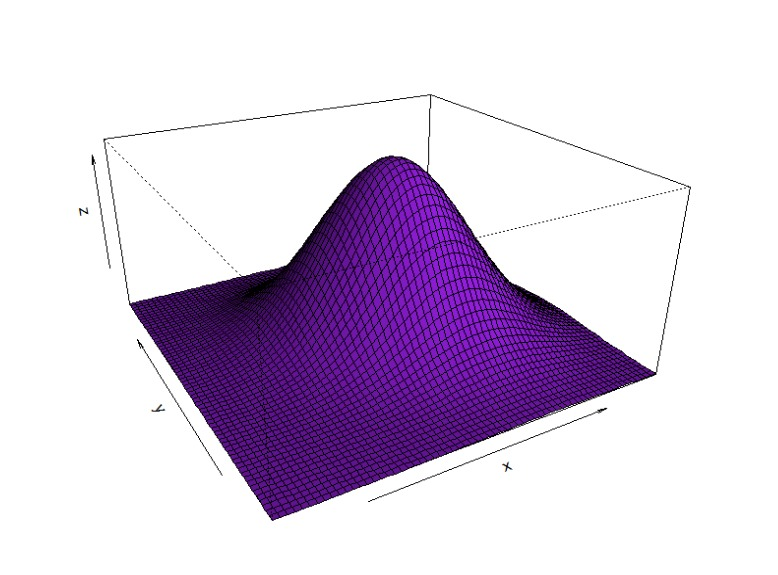
\includegraphics[width=1\linewidth]{imagenes/ej4} 


\item Encuentre la distribución condicional de $X_1$, dado $X_2$ y $X_3$. 

Conocido que $f(\mathbf{y}|\mathbf{x})$ normal multivarida con
$$E(\mathbf{y}|\mathbf{x})=\boldsymbol{\mu}_y+\boldsymbol{\Sigma}_{yx}\boldsymbol{\Sigma}_{xx}^{-1}(\mathbf{x}-\boldsymbol{\mu}_x)$$ $$cov(\mathbf{y}|\mathbf{x})=\boldsymbol{\Sigma}_{yy}-\boldsymbol{\Sigma}_{yx}\boldsymbol{\Sigma}_{xx}^{-1}\boldsymbol{\Sigma}_{xy}$$

Entonces:

$\mathbf{X}= \left[ \begin{array}{c} \mathbf{y} \\ \hline \mathbf{x} \end{array} \right]=\left[ \begin{array}{c} X_1 \\ \hline X_2 \\ X_3 \end{array} \right], \quad \quad \boldsymbol{\mu}=\left[ \begin{array}{c} \boldsymbol{\mu}_y \\ \hline \boldsymbol{\mu}_x \end{array} \right]=\left[ \begin{array}{c} 1\\ \hline 0\\ -1\end{array} \right], \quad \quad \boldsymbol{\Sigma}=\left[ \begin{array}{c|cc} \boldsymbol{\Sigma}_{yy} & \boldsymbol{\Sigma}_{yx}\\ \hline \boldsymbol{\Sigma}_{xy} & \boldsymbol{\Sigma}_{xx} \end{array} \right]=\left[ \begin{array}{c|cc} 8 & -2 & 1 \\ \hline -2 & 7 & 3 \\ 1 & 3 & 5 \end{array} \right]$

\begin{verbatim}
> muy=1
> mux=matrix(c(0,-1),ncol=1,byrow = T)
> sigmayy=8
> sigmayx=matrix(c(-2,1),ncol=2,byrow = T)
> sigmaxy=matrix(c(-2,1),ncol=1,byrow = T)
> sigmaxx=matrix(c(7,3,3,5),ncol=2,byrow = T)
> sigmayx%*%solve(sigmaxx)
     [,1] [,2]
[1,] -0.5  0.5
> cov=sigmayy-sigmayx%*%solve(sigmaxx)%*%sigmaxy
> cov
     [,1]
[1,]  6.5
\end{verbatim}

$E\left(X_1\Big|\begin{matrix}X_2 \\ X_3\end{matrix}\right)=1+\begin{bmatrix} -0.5 & 0.5\end{bmatrix}\begin{bmatrix} X_2-0 \\ X_3+1\end{bmatrix}$

$cov\left(X_1\Big|\begin{matrix}X_2 \\ X_3\end{matrix}\right)=6.5$\\

$\therefore\quad X_1\Big|\begin{matrix}X_2 \\ X_3\end{matrix} \sim N(1.5-0.5X_2+0.5X_3,6.5)$



\item Encuentre la función de densidad conjunta de $Y_1$, $Y_2$ con $Y_1 = X_1 + X_2 + X_3$, $Y_2 = X_1 - 2X_3$. 

Se tiene que $\mathbf{y}$:]
$\mathbf{y}\sim N_p(\boldsymbol{\mu},\boldsymbol{\Sigma})$; $_q\mathbf{A}_p$, $\quad \Rightarrow \quad \mathbf{A}\mathbf{y} \sim N_q(\mathbf{A}\boldsymbol{\mu},\mathbf{A}\boldsymbol{\Sigma}\mathbf{A}^t)$

Se quiere obtener la distribución conjunta de:

$\mathbf{A\underline{x}}=\begin{bmatrix} 1 & 1 & 1 \\ 1 & 0 & -2\end{bmatrix}\begin{bmatrix} X_1 \\ X_2 \\ X3 \end{bmatrix}=\begin{bmatrix} X_1+X_2+X_3 \\ X_1 -2X_3\end{bmatrix}$

\begin{verbatim}
A=matrix(c(1,1,1,1,0,-2),ncol=3,byrow=T)
mu=matrix(c(1,0,-1),ncol=1)
sigma=matrix(c(8,-2,1,-2,7,3,1,3,5),ncol=3,byrow=T)
#Media de la combinanción lineal
A%*%mu
#     [,1]
#[1,]    0
#[2,]    3
#Varianza de la combinanción lineal
A%*%sigma%*%t(A)
#     [,1] [,2]
#[1,]   24  -11
#[2,]  -11   24
\end{verbatim}

Por lo tanto, $\begin{bmatrix} Y_1 \\ Y_2 \end{bmatrix} \sim N_2 \left( \begin{bmatrix} 0\\ 3 \end{bmatrix},\begin{bmatrix} 24 & -11\\ -11 & 24 \end{bmatrix} \right)$


$\mu_1=0$, $\mu_2=3$, $\sigma_1^2 = \sigma_{11}=24$, $\sigma_2^2 = \sigma_{22}=24$, $\sigma_{12} = \sigma_{21}=-11$, $\rho_{12} = corr(y_1, y_2) = \dfrac{\sigma_{12}}{(\sigma_1 \times \sigma_2)}=\dfrac{-11}{\sqrt{24}\times\sqrt{24}}$, $\rho^2 =\left(\dfrac{-11}{\sqrt{24}\times\sqrt{24}}\right)^2=\dfrac{121}{576}$\\

La función de densidad conjunta de $Y_1$, $Y_2$ es:

$f(Y_1,Y_2)=\dfrac{1}{2\pi \sqrt{24}\sqrt{24}\sqrt{1-\dfrac{121}{576}}} \\ exp\left[ -\dfrac{1}{2\left(1-\dfrac{121}{576}\right)}\left[\left(\dfrac{Y_1-0}{\sqrt{24}}\right)^2 -2\dfrac{-11}{\sqrt{24}\sqrt{24}}\left(\dfrac{Y_1-0}{\sqrt{24}}\right)\left(\dfrac{Y_2-3}{\sqrt{24}}\right)+\left(\dfrac{Y_2-3}{\sqrt{24}}\right)^2\right]\right]$

\item Encuentre la función generadora de momentos de $Z = (Y_1, Y_2)^t$ , donde $Y_1$ y $Y_2$ son las mismas que en (d). 



Sea $\mathbf{A}$ una matrix de $r\times p$ y $\mathbf{W=AY}$ \begin{align*}
M_W(\mathbf{t})&=M_{AY}(\mathbf{t})\\
&=M_{Y}(\mathbf{A}' \mathbf{t})\\
&=e^{(\mathbf{A}' \mathbf{t})'\boldsymbol{\mu}}e^{\frac{1}{2}(\mathbf{A}' \mathbf{t})'\boldsymbol{\Sigma}(\mathbf{A}' \mathbf{t})}\\
&=e^{\mathbf{t}'(\mathbf{A}\boldsymbol{\mu})}e^{\frac{1}{2}\mathbf{t}'(\mathbf{A} 
\boldsymbol{\Sigma}\mathbf{A}') \mathbf{t}}\\
&=e^{\mathbf{t}'(\mathbf{A}\boldsymbol{\mu})+\frac{1}{2}\mathbf{t}'(\mathbf{A} 
\boldsymbol{\Sigma}\mathbf{A}') \mathbf{t}}
\end{align*}

Entonces, si $\mathbf{Z}=\begin{bmatrix} Y_1\\ Y_2 \end{bmatrix}=\mathbf{AX}=\begin{bmatrix} 1 & 1 & 1 \\ 1 & 0 & -2\end{bmatrix}\begin{bmatrix} X_1 \\ X_2 \\ X3 \end{bmatrix}=\begin{bmatrix} X_1+X_2+X_3 \\ X_1 -2X_3\end{bmatrix}$:


\begin{align*}
M_Z(\mathbf{t})&=e^{\mathbf{t}'(\mathbf{A}\boldsymbol{\mu})+\frac{1}{2}\mathbf{t}'(\mathbf{A} 
\boldsymbol{\Sigma}\mathbf{A}') \mathbf{t}}\\
&=e^{\mathbf{t}'\begin{bmatrix} 0\\ 3 \end{bmatrix}+\frac{1}{2}\mathbf{t}'\begin{bmatrix} 24 & -11\\ -11 & 24 \end{bmatrix} \mathbf{t}}
\end{align*}

\item Obtenga $P(X_1 + X_2 + 2X_3 <1.5)$

Primero se obtiene la distribución de la combinación lineal:

$\mathbf{a}^tX=\begin{bmatrix} 1 & 1 & 2 \end{bmatrix}\begin{bmatrix} X_1 \\ X_2 \\ X3 \end{bmatrix}=X_1+X_2+2X_3$

\begin{verbatim}
> a=matrix(c(1,1,2),ncol=1)
> mu=matrix(c(1,0,-1),ncol=1)
> sigma=matrix(c(8,-2,1,-2,7,3,1,3,5),ncol=3,byrow=T)
> t(a)%*%mu
     [,1]
[1,]   -1
> #Varianza 
> t(a)%*%sigma%*%a
     [,1]
[1,]   47
\end{verbatim}

$P(X_1 + X_2 + 2X_3 <1.5)$.

\begin{verbatim}
>#Probabilidad
> pnorm(1.5, mean = -1, sd = sqrt(47))
[1] 0.6423183
\end{verbatim}
\end{enumerate}


%--------EJERCICIO 5------------
\item Sea la forma cuadrática $Q:R^{2}\rightarrow R$ dada por: $q(x,y)=3x^{2}-4xy$\\

\begin{enumerate}
%----a----------
\item Dé una matriz simétrica A, para la cual: 
$q(x,y)= (x,y)A 
\begin{pmatrix}
x \\
y \\
\end{pmatrix}$\\

Para:\\
			\begin{eqnarray*}
			3x^{2}-4xy &=& (x \quad y) \cdot \begin{pmatrix}
				a&b \\
				b&c \\
			\end{pmatrix} \cdot \begin{pmatrix}
			 x\\
			 y \\
			\end{pmatrix} \\
			&=&(x \quad y) \cdot \begin{pmatrix}
				ax+by \\
				bx+cy \\
			\end{pmatrix}\\
			&=&(ax+by)x+(bx+cy)y\\
			&=&ax^{2}+2bxy+cy^{2}
		\end{eqnarray*}
		con:
		\begin{eqnarray*}
			a &=& 3\\
			2b&=&-4 \quad \Rightarrow \quad b=-2\\
			c&=&0
		\end{eqnarray*}
		
			$A= \begin{pmatrix}
				3 & -2 \\
				-2 & 0 \\
			\end{pmatrix}$
			
	

%--------b---------
\item ¿Qué tipo de definifitividad tiene $Q$?\\

Criterio de clasificación de autovalores:\\
\begin{verbatim}
> a=matrix ( c(3 , -2 , -2 ,0) , nrow = 2 , ncol = 2 )
> e=eigen(A)
> e
eigen() decomposition
$values
[1]  4 -1

$vectors
           [,1]       [,2]
[1,] -0.8944272 -0.4472136
[2,]  0.4472136 -0.8944272
\end{verbatim}
Dado que valor propio es 4 positivo y  -1 negativo, la forma cuadrática es indefinida.

%-------c----------------------
\item Grafique $Q$
\begin{verbatim}
Q <- function(x, y) {3 * x^2 - 4 * x * y}
x <- seq(-10, 10, length.out = 100)
y <- seq(-10, 10, length.out = 100)
z <- outer(x, y, Q)
persp(x,y,z,theta = 30, phi=30, col="pink",expand=0.5, r=2,ltheta=25)
\end{verbatim}
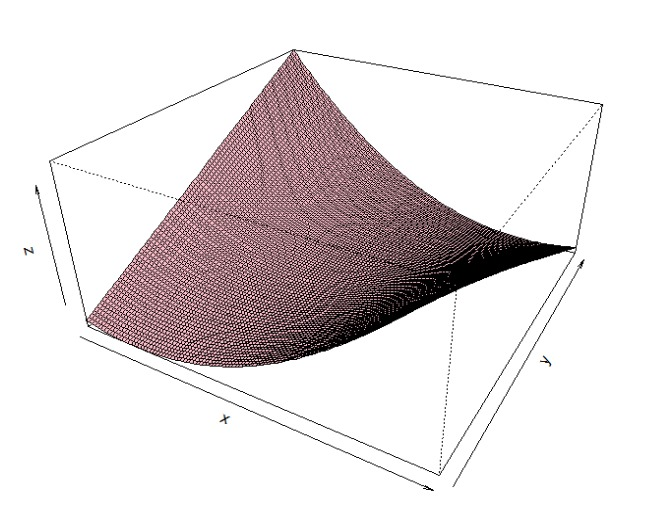
\includegraphics[width=0.7\linewidth]{imagenes/ej5} 
\end{enumerate}

\end{enumerate}
\end{document}